%\newpage
%\pagestyle{empty}

\chapter{INTRODUÇÃO}{}
%\thispagestyle{empty}
%\pagestyle{fancy}
\section{Considerações Iniciais}
A crescente demanda por energia elétrica no decorrer dos anos impulsionou o desenvolvimento de novas tecnologias voltadas para análise e monitoramento, com o propósito de promover uma gestão mais eficiente do consumo energético. Nesse sentido, as diretrizes estabelecidas pela Agência Nacional de Energia Elétrica no Módulo 8 do PRODIST – Procedimentos de Distribuição de Energia Elétrica no Sistema Elétrico Nacional preveem grandezas elétricas como corrente, tensão e fator de potência como parâmetros essenciais para a análise do comportamento de cargas e para futuras otimizações no uso da energia elétrica\cite{ANEEL2021}.

Nesse viés, atualmente, com os avanços associados à Indústria 4.0, tecnologias voltadas à aquisição e ao processamento de dados em tempo real, aliadas ao baixo custo e ao reduzido consumo de energia, tornaram-se fundamentais para a leitura e coleta de informações relacionadas ao comportamento do consumo energético em diferentes aplicações, especialmente no que se refere à qualidade da energia elétrica. Desse modo, o emprego de plataformas embarcadas tem se mostrado uma alternativa eficiente para a implementação de sistemas de monitoramento elétrico\cite{Gilchrist2016}.

Ademais, o crescimento do volume de dados gerados por sistemas de monitoramento abre espaço para a aplicação de técnicas de aprendizado de máquina. Métodos de análise baseados em machine learning permitem identificar padrões e tendências em grandes conjuntos de dados, possibilitando a previsão do consumo energético e auxiliando na tomada de decisões relacionadas à gestão da energia\cite{Bishop2006}. Essa abordagem tem sido investigada em estudos recentes devido ao seu potencial de melhorar a eficiência energética em diversos setores.

Além disso, a ocorrência de variações e interrupções no fornecimento de energia elétrica pode ocasionar danos a equipamentos eletroeletrônicos. Em muitas ocasiões, consumidores enfrentam dificuldades para comprovar essas ocorrências junto às concessionárias de energia elétrica, uma vez que não possuem registros detalhados das condições do fornecimento no momento do evento. 

Diante do exposto, este trabalho tem por objetivo o desenvolvimento de um sistema embarcado para monitoramento de grandezas elétricas associadas ao consumo energético, aliado à aplicação de técnicas de \textit{machine learning} para análise dos dados coletados e previsão do consumo de energia. Assim, a solução proposta será capaz de identificar padrões de consumo, estimar demandas futuras de energia e registrar informações que auxiliem na análise de possíveis variações ou interrupções no fornecimento de energia elétrica.

\section{Objetivo Geral}
Desenvolver um sistema embarcado capaz de realizar o monitoramento de grandezas elétricas, como tensão e corrente, permitindo a análise de parâmetros associados ao consumo energético, aliado à aplicação de técnicas de \textit{machine learning} para análise dos dados coletados e previsão do consumo de energia para ambientes residenciais.

\section{Objetivos Específicos}
\begin{itemize}
    \item Projetar e implementar um sistema embarcado para aquisição de dados de tensão e corrente elétrica.
    \item Realizar o monitoramento e registro contínuo das grandezas elétricas, possibilitando a identificação de variações e eventuais interrupções no fornecimento de energia.
    \item Processar os sinais elétricos medidos para obtenção de parâmetros como tensão eficaz, corrente eficaz, potência ativa, potência reativa, potência aparente e fator de potência.
    \item Armazenar e organizar os dados coletados para posterior análise do comportamento do consumo energético.
    \item Desenvolver um modelo preditivo capaz de estimar o consumo energético com base nos dados coletados.
    \item Avaliar o desempenho do sistema desenvolvido, verificando sua capacidade de monitoramento, registro de eventos e previsão do consumo de energia.
\end{itemize}

\section{Metodologia do Trabalho}
Neste trabalho, será desenvolvido um sistema embarcado voltado para aplicações de segurança, utilizando sensores para aquisição de dados e um microcontrolador responsável pelo processamento das informações. O sistema será projetado com o objetivo de monitorar eventos em tempo real e identificar possíveis situações de risco por meio dos valores de grandezas elétricas coletadas. As etapas descritas serão organizadas de forma sequencial, permitindo uma compreensão clara do funcionamento do sistema proposto ao longo do desenvolvimento do trabalho.

Em concordância com a Figura \ref{fig:03}, a metodologia de desenvolvimento do trabalho será estruturada em três etapas principais.

\begin{figure}[!h]
    \centering
    \caption{Diagrama de blocos do sistema proposto}
    % A professora pediu para aumentar a figura (width alterado de 12cm para 15cm)
    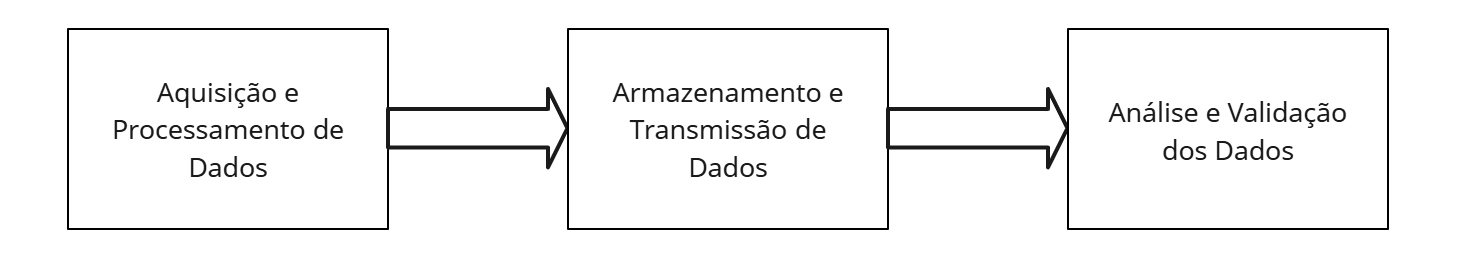
\includegraphics[width=15cm]{figuras/Diagrama_met.png}\\
    \autoria{Autoria Própria}
    \label{fig:03}
\end{figure}

\begin{enumerate}
\renewcommand{\labelenumi}{\Roman{enumi}.}
\item Inicialmente, será realizada a etapa de aquisição de dados, na qual os sensores serão utilizados para captar as variáveis de interesse do ambiente monitorado. Em seguida, os dados obtidos serão processados pelo microcontrolador, utilizando algoritmos específicos para análise e tomada de decisão, permitindo a identificação de padrões ou condições anormais.
\item Posteriormente, os resultados processados poderão ser armazenados ou transmitidos, possibilitando o registro das informações e o acompanhamento do sistema.
\item Por fim, será realizada a análise dos dados obtidos, visando validar o funcionamento do sistema e avaliar sua eficiência na detecção de eventos de interesse.
\end{enumerate}

\section{Organização do Texto}

\textbf{Capítulo 2} - É apresentada uma revisão bibliográfica sobre os principais conceitos relacionados ao tema, reunindo os trabalhos que fundamentam o desenvolvimento desta pesquisa.

\textbf{Capítulo 3} - É apresentada a fundamentação teórica do trabalho, abordando conceitos sobre arquiteturas de microcontroladores, conversão analógico-digital, aquisição e condicionamento de sinais, Teorema de Nyquist-Shannon, grandezas elétricas em sistemas digitais, qualidade de energia elétrica e técnicas de aprendizado de máquina empregadas neste estudo.

\textbf{Capítulo 4} - Neste capítulo é apresentada a metodologia adotada para o desenvolvimento do sistema proposto, apresentando os materiais, métodos e etapas de desenvolvimento utilizados na implementação e validação do sistema proposto.

\textbf{Capítulo 5} - Apresenta os resultados parciais obtidos

\textbf{Capítulo 6} - Apresenta as considerações finais do trabalho.
%\newpage
%\thispagestyle{empty}